\documentclass[9pt]{beamer}
\usepackage{tikz}
\usepackage{subfiles}
\usepackage{graphicx} 
\usepackage{hyperref}
\usepackage{multimedia}
\usepackage{subcaption}
%\usepackage[table,xcdraw]{xcolor}  %to include tables with colors

\setbeamertemplate{footline}[page number]
\mode<presentation>{
%\usetheme{Malmoe}
%\usetheme{Antibes}
%\usetheme{warsaw}
\usetheme{Frankfurt}  %%
%\usetheme{Dresden}
%\usetheme{Madrid}
%\usetheme{Malmoe} %
%\usetheme{Ilmenau}
}
%\setbeamertemplate{footline}[\insertframenumber]

%\newcommand*\oldmacro{}%
%\let\oldmacro\insertshorttitle%
%\renewcommand*\insertshorttitle{%
% \oldmacro\hfill%
% \insertframenumber\,/\,\inserttotlaframenumber}

\AtBeginSection[]
{
\begin{frame}<beamer>
\frametitle{Plan}
\tableofcontents[currentsection]
\end{frame}
}

\begin{document}
\title[FEM on plates]{FEM in plates}
\author{Emaya}
\institute[ECN]


\begin{frame}
\titlepage
\end{frame}

\begin{frame}
\frametitle{Plan}
\begin{figure}[h!]
%\centering
%\minipage{1\textwidth}%
  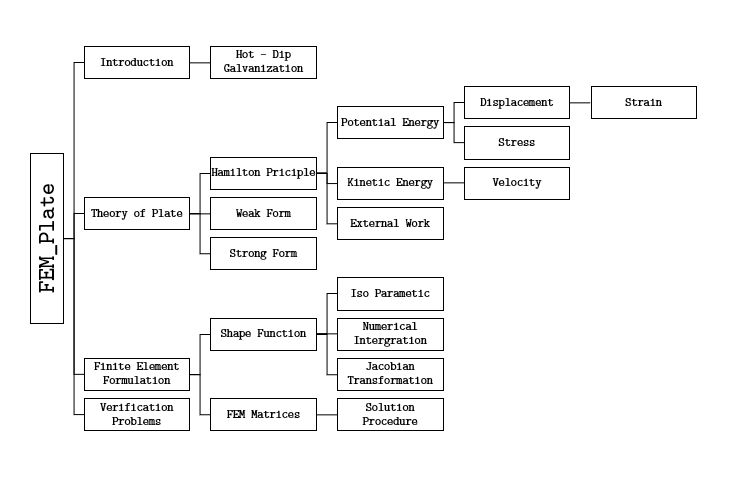
\includegraphics[width=1\linewidth,trim={0 0 0 1cm},clip]{tree.png}
 % \caption{FEM solution plot}\label{fig:awesome_image3}
%\endminipage
\end{figure}
\end{frame}

\begin{frame}
\frametitle{Table of Content}
\tableofcontents
\end{frame}
\section{Introduction}
\begin{frame}
\frametitle{Introduction}
\end{frame}
\subsection{Hot-Dip Galvanization Process}
\begin{frame}
\frametitle{Hot-Dip Galvanization Process}
\begin{columns}
\column{0.5\textwidth}

\begin{figure}[h!]
%\centering
%\minipage{1\textwidth}%
  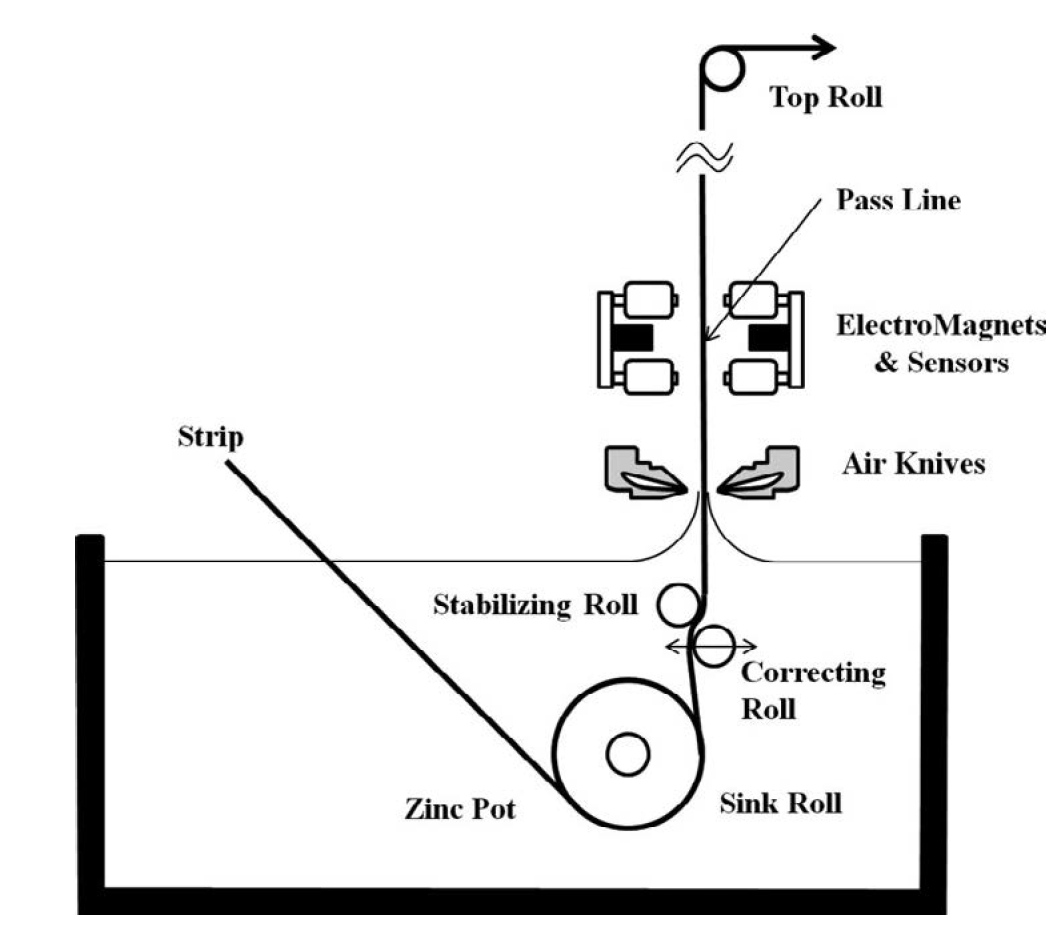
\includegraphics[width=1\linewidth,trim={0 0 0 1cm},clip]{hotdip.png}
 % \caption{FEM solution plot}\label{fig:awesome_image3}
%\endminipage
\end{figure}
\column{0.5\textwidth}
\begin{itemize}
\item A thin Layer of Zinc is coated to Increase the corrosion resistance of steel
\item Air knives control the thickness of the Zinc layer
\item Excessive Vibration results in uneven coating.
\item Electromagnets are used to control vibration of the strip. 
\end{itemize}
\end{columns}
\end{frame}




\begin{frame}
\frametitle{Need For Finite Element Modeling}

\begin{itemize}
\item Complex behavior of the metal strip.
\item Two dimensional domain and Three Dimensional Displacement field.
\item Complex and multiple boundary condition.
\item Free Control over discretization of the domain.
\item Intuitive Solution Procedure.
\end{itemize}

\end{frame}

\section{Theory of Plates}
\begin{frame}
\frametitle{Theory of Plates}
A plate is a flat solid with uniform and smaller thickness than its other dimensions.A middle plane (Z=0) is equidistant from upper and lower faces.
\begin{block}{Assumptions}
\begin{itemize}
\item A point in the middle plane only moves vertically $u = 0$ and $v = 0 $
\item Thickness does not change during deformation.
\item $\sigma_{33}$ is neglected (plane stress is assumed)
\end{itemize}
\end{block}

\begin{figure}[h!]
%\centering
%\minipage{1\textwidth}%
  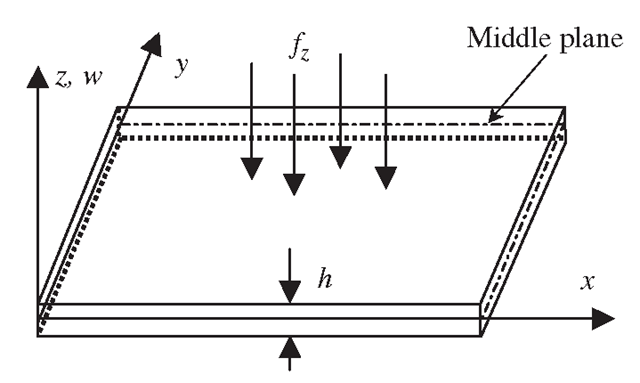
\includegraphics[width=0.5\linewidth,trim={0 0 0 1cm},clip]{plate.png}
 % \caption{FEM solution plot}\label{fig:awesome_image3}
%\endminipage
\end{figure}

\end{frame}

\begin{frame}
\frametitle{Theory of Plates}
\begin{block}{Kirchhoff Plate Theory}
\begin{itemize}
\item A line normal to the undeformed middle plane remains straight and normal after deformation.
\item Only for \textbf{Thin Plates} where $t/a \leq 0.1 $.
\item $\sigma_{23}$ and $\sigma_{13}$ are neglected.
\end{itemize}
\end{block}


\begin{figure}[h!]
%\centering
%\minipage{1\textwidth}%
  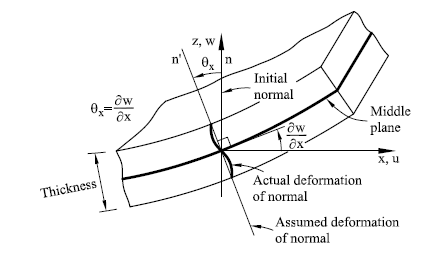
\includegraphics[width=0.6\linewidth,trim={0 0 0 0},clip]{Kplate.png}
 % \caption{FEM solution plot}\label{fig:awesome_image3}
%\endminipage
\end{figure}

\end{frame}


\begin{frame}
\frametitle{Theory of Plates}

\begin{block}{Reissner-Mindlin Plate Theory}
\begin{itemize}
\item A line normal to the undeformed middle plane remains straight and not necessarily normal after deformation.
\item For both \textbf{Thin and Thin Plates}.
\item $\sigma_{23}$ and $\sigma_{13}$ are not neglected.
\end{itemize}
\end{block}


\begin{figure}[h!]
%\centering
%\minipage{1\textwidth}%
  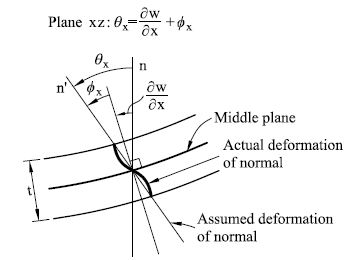
\includegraphics[width=0.6\linewidth,trim={0 0 0 0},clip]{RMplate.png}
 % \caption{FEM solution plot}\label{fig:awesome_image3}
%\endminipage
\end{figure}

\end{frame}

\begin{frame}
\frametitle{Description of Domain}

\begin{figure}[h!]
\centering
\subfile{domain.tex}
%\caption{NAS277} \label{NAS277sch}
\end{figure}
\begin{columns}
\column{0.5\textwidth}

\begin{equation*}
\Omega \in \left\{ x, y \right\}
\end{equation*}
\begin{equation*}
\Gamma \in \left\{ \Omega \times z \right\}
\end{equation*}
\begin{equation*}
z \in \left\{ -\frac{t}{2}, \frac{t}{2} \right\}
\end{equation*}
\end{columns}

\end{frame}

\subsection{Hamilton Principle}
\begin{frame}
\frametitle{Hamilton principle}
Hamilton principle is used to derive the equation of motion. 
 
 \begin{align*}
H & = \int_{t_0}^{t_1} \left( T - V + W \right) dt &  \\
 \delta H & =  \int_{t_0}^{t_1} \left( \delta T - \delta V + \delta W \right) dt   &  =  0 
\\
 &\delta u \Big|_{t_0}^{t_1}& = 0
 \end{align*}
 $T$ is the kinetic energy, $V$ in the potential energy and $W$ is the work done to the system.
 
\end{frame}
\subsection{Potential Energy}
\begin{frame}
\frametitle {Potential Energy}

\begin{equation*}
V=\frac{1}{2}\int\int\int_\Gamma \epsilon^T \sigma  d \Gamma
\end{equation*}

\begin{equation*}
V=\frac{1}{2}\int\int\int_\Gamma \left(\epsilon^B\right)^T \sigma^B + \left(\epsilon^S\right)^T \sigma^S + \left(\epsilon^A\right)^T \sigma^A d \Gamma
\end{equation*}

\begin{equation*}
V=\frac{1}{2}\int\int_\Omega \int_{-t/2}^{+t/2} \left(\epsilon^B\right)^T \sigma^B + \left(\epsilon^S\right)^T \sigma^S + \left(\epsilon^A\right)^T \sigma^A dz d \Omega
\end{equation*}

$\epsilon^B$ is the stress due to bending, $\epsilon^S$ is the stress due to shear deformation and  $\epsilon^A$ is the axial stress.

\end{frame}

\begin{frame}
\frametitle{Kinematics}
\begin{align*}
u_1 \left( x, y ,z,t\right) & =  u \left( x ,y,t\right) - z \theta_x \left(x,y,t\right) & \theta_x  = \frac{\partial w }{\partial x} + \phi_x \\
u_2 \left( x, y ,z,t\right) & =  v \left( x, y ,t\right) - z \theta_y \left(x,y,t\right)& \theta_y  = \frac{\partial w }{\partial y} + \phi_y\\
u_3 \left( x, y ,z,t\right) & =  w \left(x, y ,t\right) 
\end{align*}
\begin{columns}
\column{0.65\textwidth}
\begin{equation*}
\left\{
\begin{array}{r}
 u_1 \\ u_2 \\ u_3  
\end{array}
\right\}
=
\begin{bmatrix}
z & 0 & 0 \\
0 & z & 0 \\
0 & 0 & 1 \\
\end{bmatrix}
\left\{
\begin{array}{r}
 \theta_x \\ \theta_y \\ w 
\end{array}
\right\}
=
\left[Z \right] \tilde{u}
\end{equation*}
\column{0.35\textwidth}
\begin{figure}[h!]
%\centering
%\minipage{1\textwidth}%
  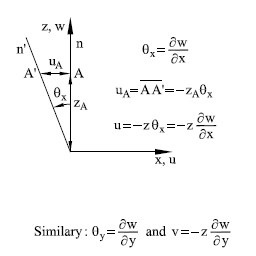
\includegraphics[width=1\linewidth,trim={0 2cm 0 0},clip]{displacement.png}
 % \caption{FEM solution plot}\label{fig:awesome_image3}
%\endminipage
\end{figure}
\end{columns}

\end{frame}


\begin{frame}
\frametitle{Strain Definition}
The Green - Lagrange strain tensor is given as
\begin{equation*}
\epsilon_{ij} = \frac{1}{2} \left(  u_{i,j} +  u_{j,i} + u_{k,i}u_{k,j} \right) \qquad i,j \in 1,2,3
\end{equation*}


The $E_{11}$ component of the strain tensor is found as
\begin{align*}
E_{11} = -z \dfrac{\partial w^2 }{\partial x^2} + \dfrac{1}{2}\left(\left[z\dfrac{\partial \theta_x}{\partial x}\right] ^2 +z^2 \dfrac{\partial \theta_y}{\partial x}\dfrac{\partial \theta_y}{\partial y} + \dfrac{\partial w}{\partial x} \dfrac{\partial w}{\partial x}\right)
\end{align*}

\begin{align*}
E_{11} = -z \dfrac{\partial w^2 }{\partial x^2} + \dfrac{1}{2} \left( \dfrac{\partial w}{\partial x} \right)^2
\end{align*}
\end{frame}

\begin{frame}
\begin{align*}
E_{i,j} =  
\begin{bmatrix}
 -z \dfrac{\partial w^2 }{\partial x^2} + \dfrac{1}{2} \left( \dfrac{\partial w}{\partial x} \right)^2
 & 
 -z \dfrac{\partial w^2 }{\partial x \partial y} + \dfrac{1}{2}  \dfrac{\partial w}{\partial x} \dfrac{\partial w}{\partial y} 
 & 
 \dfrac{1}{2} \left( \dfrac{\partial w}{\partial x}-\theta_x \right)
 \\
 &
 -z \dfrac{\partial w^2 }{\partial y^2} + \dfrac{1}{2} \left( \dfrac{\partial w}{\partial y} \right)^2
 &
  \dfrac{1}{2} \left( \dfrac{\partial w}{\partial y}-\theta_y \right)
  \\
  symm.
  &
  &
  0
\end{bmatrix}
\end{align*}



\begin{align*}
\epsilon_{\alpha \beta}^B = -z
\begin{bmatrix}
\dfrac{\partial w^2 }{\partial x^2}
\\
\dfrac{\partial w^2 }{\partial y^2}
\\
\dfrac{\partial w^2 }{\partial x \partial y}
\end{bmatrix}
=-z \kappa
  \quad  \alpha,\beta\in 1,2
\end{align*}
$\kappa= \mathbf{\triangledown} w$ is the curvature of of a plane.
\end{frame}
\begin{frame}
\begin{align*}
\epsilon_{\alpha \beta}^A = \dfrac{1}{2}
\begin{bmatrix}
 \left( \dfrac{\partial w}{\partial x} \right)^2 
 &
 \dfrac{\partial w}{\partial x}\dfrac{\partial w}{\partial y}  
\\
 \dfrac{\partial w}{\partial x}\dfrac{\partial w}{\partial y} 
 &
 \left( \dfrac{\partial w}{\partial y} \right)^2
\end{bmatrix}
=
\frac{1}{2}
\begin{bmatrix}
\dfrac{\partial w}{\partial x} \\
\dfrac{\partial w}{\partial y}
\end{bmatrix}
\begin{bmatrix}
\dfrac{\partial w}{\partial x} &
\dfrac{\partial w}{\partial y}
\end{bmatrix}
\end{align*}
\begin{align*}
\epsilon_{3\alpha}^S = \dfrac{1}{2}
\begin{bmatrix}
\dfrac{\partial w}{\partial x}-\theta_x 
\\
\dfrac{\partial w}{\partial y}-\theta_y 
\end{bmatrix} 
\end{align*}
\begin{columns}
\column{0.5\textwidth}
For Kirchhoff plate
\begin{align*}
\epsilon_{3\alpha}^S =
\begin{bmatrix}
0
\\
0 
\end{bmatrix} 
\end{align*}
\column{0.5\textwidth}
For Reissner - Mindlin Plate
\begin{align*}
\epsilon_{3\alpha}^S = \dfrac{1}{2}
\begin{bmatrix}
-\phi_x 
\\
-\phi_y 
\end{bmatrix} 
\end{align*}
\end{columns}
\end{frame}

\begin{frame}
\frametitle{Constitute law}
For the \textbf{linear isotropic} material is considered. Since $\sigma_{33}$ is not considered the \textbf{plane stress} case is considered and the stress - strain relation is given as
\begin{equation*}
\sigma_{\alpha\beta}^B = \begin{bmatrix}
\sigma_{11}
\\
\sigma_{22}
\\
2 \sigma_{12}
\end{bmatrix}
=\dfrac{1}{1-\nu^2}
\begin{bmatrix}
E & \nu E & 0
\\
\nu E & E & 0
\\
0 & 0 & (1-\nu^2)G
\end{bmatrix}
\begin{bmatrix}
\epsilon_{11}
\\
\epsilon_{22}
\\
2 \epsilon_{12}
\end{bmatrix}
\end{equation*}



$E$ is the Young's modulus, $\nu$ is the Poisson's ratio and $G$ is the shear modulus which is given by $G=E / 1+\nu $. 
\begin{equation*}
\sigma_{\alpha\beta}^B = \mathbf{D} \epsilon_{\alpha\beta}^B
\end{equation*}
\end{frame}


\begin{frame}

The shear stress and strain relation from the 3D constitutive law is given as
\begin{equation*}
\sigma_{3\alpha}^S = \begin{bmatrix}
2 \sigma_{31}
\\
2 \sigma_{32}
\end{bmatrix}
=G
\begin{bmatrix}
1 & 0 
\\
0 & 1 
\end{bmatrix}
\begin{bmatrix}
2\epsilon_{31}
\\
2\epsilon_{32}
\end{bmatrix}
=
\mathbf{D_c}
\sigma_{3\alpha}^S
\end{equation*}

Axial is stress is provided and it is considered as constant and uniform over the domain.

\begin{equation*}
\sigma_{\alpha\beta}^A = \begin{bmatrix}
\sigma_{11} & \sigma_{12}
\\
\sigma_{12} & \sigma_{22}
\end{bmatrix}
=
\begin{bmatrix}
N_x & N_{xy}
\\
N_{xy} & N_y
\end{bmatrix}
=
N
\end{equation*}

\end{frame}

\begin{frame}
\begin{equation*}
V=\frac{1}{2}\int\int_\Omega \int_{-t/2}^{+t/2} \left(\epsilon^B\right)^T \sigma^B + \left(\epsilon^S\right)^T \sigma^S + \left(\epsilon^A\right)^T \sigma^A dz d \Omega
\end{equation*}

\begin{equation*}
\begin{split}
V=\frac{1}{2} \int\int_\Omega
\left[ \int_{-t/2}^{+t/2} z^2 dz\right]
  \kappa^T D  \kappa 
+ \left[ \int_{-t/2}^{+t/2} dz\right]\left(\tilde{\epsilon}^S\right)^T {D_c} \tilde{\epsilon}^S \\
+ \left[ \int_{-t/2}^{+t/2} dz\right]
 \left(\tilde{\epsilon}^A\right)^T \sigma^A  d \Omega
\end{split}
\end{equation*}
\begin{equation*}
\begin{split}
V=\frac{1}{2} \int\int_\Omega  \kappa^T \tilde{D}  \kappa 
+ \left(\tilde{\epsilon}^S\right)^T {\tilde{D}_c} \tilde{\epsilon}^S 
+ \left(\tilde{\epsilon}^A\right)^T \tilde{\sigma}^A  d \Omega
\end{split}
\end{equation*}
\begin{equation*}
\begin{split}
 \tilde{D} = \frac{t^3}{12}D \quad \tilde{D}_c = t{D}_c 
\quad \tilde{\sigma}^A  = t{\sigma}^A
\end{split}
\end{equation*}
\end{frame}

\begin{frame}

\begin{equation*}
\begin{split}
\delta V=\int\int_\Omega  \kappa^T \tilde{D}  \delta \kappa 
+ \left(\tilde{\epsilon}^S\right)^T {\tilde{D}_c}  \delta \tilde{\epsilon}^S 
+ \frac{1}{2} \left( \delta  \tilde{\epsilon}^A\right)^T \tilde{\sigma}^A  d \Omega
\end{split}
\end{equation*}


\begin{equation*}
\frac{1}{2} \left( \delta  \tilde{\epsilon}^A\right)^T \tilde{\sigma}^A =
w_{, \alpha} \tilde{\sigma}^A  \delta w_{, \alpha}
\end{equation*}

\begin{block}{Variation of Total Potential Energy}
\begin{equation*}
\begin{split}
\delta V=\int\int_\Omega  \kappa^T \tilde{D}  \delta \kappa 
+ \left(\tilde{\epsilon}^S\right)^T {\tilde{D}_c}  \delta \tilde{\epsilon}^S 
+ w_{, \alpha} \tilde{\sigma}^A  \delta w_{, \alpha}  d \Omega
\end{split}
\end{equation*}

\end{block}
\end{frame}

\subsection{Kinetic Energy}

\begin{frame}
\frametitle{Kinetic Energy}
The kinetic of a material is given as
\begin{equation*}
T = \frac{1}{2} \int \int \int_{\Gamma} \mathbf{v}^T\rho\mathbf{v} d\Gamma
\end{equation*}
For plate, the integration along thickness is done now.
\begin{equation*}
T = \frac{1}{2} \int \int_\Omega \left[ \int_{-\frac{t}{2}}^{\frac{t}{2}} \mathbf{v}^T\rho\mathbf{v} dz \right] d\Omega
\end{equation*}

\end{frame}


\begin{frame}
\frametitle{Description of velocity}

\begin{columns}
\column{0.3\textwidth}
\begin{block}{Lagrangian}
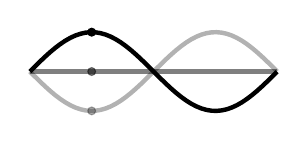
\begin{tikzpicture}[scale=0.5]

\draw [ultra thick,domain=0:2*3.14, samples=50] plot (\x, {+sin(\x r)});
\draw [ultra thick,domain=0:2*3.14, samples=50,opacity=0.5] plot (\x, {0});
\draw [ultra thick,domain=0:2*3.14, samples=50,opacity=0.3] plot (\x, {-sin(\x r)});

\draw[fill=black] (3.14*0.5,1,0) circle (0.1 );
\draw[fill=black,opacity=0.5] (3.14*0.5,0,0) circle (0.1 );
\draw[fill=black,,opacity=0.3] (3.14*0.5,-1,0) circle (0.1 );
 \end{tikzpicture}
 \begin{itemize}
 \item Material Point moves along with spatial point
 \item Used for solids
 \end{itemize}
\end{block}

\column{0.3\textwidth}
\begin{block}{Eulerian}


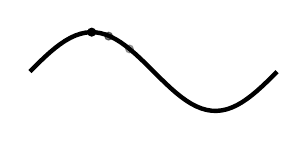
\begin{tikzpicture}[scale=0.5]

\draw [ultra thick,domain=0:2*3.14, samples=50] plot (\x, {3+sin(\x r)});
%\draw [ultra thick,domain=0:2*3.14, samples=50,opacity=0.7] plot (\x, {0});
%\draw [ultra thick,domain=0:2*3.14, samples=50,opacity=0.3] plot (\x, {-sin(\x r)});

\draw[fill=black] (3.14*0.5,3+1,0) circle (0.1 );
\draw[fill=black,opacity=0.5] (2,3+0.9,0) circle (0.1 );
\draw[fill=black,,opacity=0.3] (2.53,3+0.574,0) circle (0.1 );



 \end{tikzpicture}
 \begin{itemize}
 \item Material Point moves but spatial point stays
 \item Used for fluids
 \end{itemize}
 
 \end{block}
\column{0.3\textwidth}
\begin{block}{Mixed}


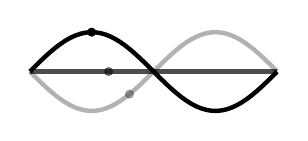
\begin{tikzpicture}[scale=0.5]


\draw [ultra thick,domain=0:2*3.14, samples=50] plot (\x, {-3+sin(\x r)});
\draw [ultra thick,domain=0:2*3.14, samples=50,opacity=0.7] plot (\x, {-3});
\draw [ultra thick,domain=0:2*3.14, samples=50,opacity=0.3] plot (\x, {-3-sin(\x r)});

\draw[fill=black] (3.14*0.5,-3+1,0) circle (0.1 );
\draw[fill=black,opacity=0.5] (2,-3,0) circle (0.1 );
\draw[fill=black,,opacity=0.3] (2.53,-3-0.574,0) circle (0.1 );

 \end{tikzpicture}
 \begin{itemize}
 \item Both point moves independently.
 \item Moving Material
 \end{itemize}
 
 \end{block}
 
\end{columns}
\begin{block}{Material Derivative}


\begin{equation*}
\frac{d(\circ)}{dt}=\frac{\partial(\circ)}{\partial t} + V_i \cdot (\circ)_{,i} 
\end{equation*}
\begin{equation*}
  v_i = \dot{u_i}+V_1u_{i,1}
\end{equation*} 

\end{block}

\end{frame}



\begin{frame}
%\frametitle{Variation of the kinetic energy}
First the integration along thickness is done
\begin{equation*}
\int_{-\frac{t}{2}}^{\frac{t}{2}} \mathbf{v}^T\rho\mathbf{v} dz =
\int_{-\frac{t}{2}}^{\frac{t}{2}}
\left(
\rho\dot{u_i}\dot{u_i}
+
2 \rho V_1 \dot{u_i} u_{i,1}
+
\rho V_1^2 u_{i,1} u_{i,1}
\right) dz
\end{equation*}
\begin{equation*}
 =
\rho \dot{\tilde{u_i}} Z_{ij} \dot{\tilde{u_i}}
+
2 \rho V_1 \dot{\tilde{u_i}} Z_{ij} \tilde{u}_{j,1} 
+
\rho V_1^2 \tilde{u}_{j,1} Z_{ij} \tilde{u}_{j,1}
\end{equation*}
substituting it in the kinetic energy equation
\begin{equation*}
T = \frac{1}{2} \int \int_\Omega \left(
\rho \dot{\tilde{u_i}} Z_{ij} \dot{\tilde{u_i}}
+
\rho V_1 \dot{\tilde{u_i}} Z_{ij} \tilde{u}_{j,1} 
+
\rho V_1^2 \tilde{u}_{j,1} Z_{ij} \tilde{u}_{j,1}
 \right) d\Omega
\end{equation*}
\begin{columns}
\column{0.7\textwidth}
\begin{block}{Variations of Kinetic Energy}


\begin{equation*}
\begin{split}
\delta T = & \int \int_\Omega 
\rho \dot{\tilde{u_i}} Z_{ij} \delta \dot{\tilde{u_i}}
+
\rho V_1 \delta \dot{\tilde{u_i}} Z_{ij} \tilde{u}_{j,1} \\ &
  +  
\rho V_1  \dot{\tilde{u_i}} Z_{ij} \delta \tilde{u}_{j,1} 
+
\rho V_1^2 \tilde{u}_{j,1} Z_{ij} \delta \tilde{u}_{j,1}
 d\Omega
\end{split}
\end{equation*}

\end{block}

\column{0.3\textwidth}
\begin{equation*}
Z_{ij}=
\begin{bmatrix}
\frac{t^3}{12} & 0 & 0 \\
0 & \frac{t^3}{12} &  0 \\
0 &   0 & t 
\end{bmatrix}
\end{equation*}
\end{columns}

\end{frame}



\subsection{External Work}
\begin{frame}
\frametitle{External Work}
more summation and write them separately for variations. 
\begin{equation*}
 W=\sum_i^{nb} W_i=\sum_i^{nb} \int_{\Omega_i} q_i \mathbf{ u_i}  d \Omega_i
\end{equation*}

\begin{block}{Variation of the external work}
\begin{equation*}
\delta W=\sum_i^{nb} \int_{\Omega_i} q_i \mathbf{\delta u_i}  d \Omega_i
\end{equation*}
\end{block}



\end{frame}


\begin{frame}
\frametitle{The Hamilton principle} 
Substituting Everything in Hamilton principle gives
\begin{equation*}
\begin{split}
 \int_{t_0}^{t_1} \left( \delta T - \delta V + \delta W \right) dt    =  0 
\end{split} 
\end{equation*}
\begin{equation*}
\begin{split}
 \int \int_\Omega 
+
\rho \dot{\tilde{u_i}} Z_{ij} \delta \tilde{u_i}
+
\rho V_1 \delta {\tilde{u_i}} Z_{ij} \tilde{u}_{j,1} 
+  
\rho V_1 {\tilde{u_i}} Z_{ij} \delta \tilde{u}_{j,1}  
 d \Omega  \Big|_{t_0}^{t_1} 
 \\ 
 \int_{t_0}^{t_1} \int \int_\Omega 
-
\rho \ddot{\tilde{u_i}} Z_{ij} \delta {\tilde{u_i}}
-
\rho V_1 \delta {\tilde{u_i}} Z_{ij} \dot{\tilde{u}}_{j,1} 
-  
\rho V_1  \tilde{u_i} Z_{ij} \delta \dot{\tilde{u}}_{j,1} 
+
\rho V_1^2 \tilde{u}_{j,1} Z_{ij} \delta \tilde{u}_{j,1}
\\ 
- 
\kappa^T \tilde{D} \delta\kappa 
-
\left(\epsilon^S\right)^T \tilde{D_c} \delta\epsilon^S 
- 
 w_{, \alpha} \tilde{\sigma}^A  \delta w_{, \alpha}  d \Omega     \\
 +   
 \sum_i^{nb}   \int  \int_{\Omega_i} q_i \mathbf{\delta u_i}  d \Omega_i dt = 0
\end{split} 
\end{equation*}
\end{frame}

\begin{frame}
\frametitle{Weak Form}
$
\int_{t_0}^{t_1} \chi dt = 0
$
For this to be true
$
 \chi  = 0
$  must also be true
\begin{block}{Final Weak Form}

\begin{equation*}
\begin{split}
 \int \int_\Omega 
\rho \ddot{\tilde{u_i}} Z_{ij} \delta {\tilde{u_i}}
+
2 \rho V_1 \delta {\tilde{u_i}} Z_{ij} \dot{\tilde{u}}_{j,1} 
-
\rho V_1^2 \tilde{u}_{j,1} Z_{ij} \delta \tilde{u}_{j,1}
\\ 
+
\kappa^T \tilde{D} \delta\kappa 
+
\left(\epsilon^S\right)^T \tilde{D_c} \delta\epsilon^S 
+ 
 w_{, \alpha} \tilde{\sigma}^A  \delta w_{, \alpha} d \Omega     \\
=  
 \sum_i^{nb}   \int  \int_{\Omega_i} q_i \mathbf{\delta u_i}  d \Omega_i dt
\end{split} 
\end{equation*}

\end{block}
\end{frame}

\begin{frame}
\frametitle{Weak Form}
$
\int \int_\Omega \chi d\Omega = 0
$
For this to be true
$
 \chi  = 0
$  must also be true and by considering $\epsilon^S=0$, $\tilde{\sigma}^A=N_x$ and $\tilde{u}_1 =\tilde{u}_2 = 0 $ we get the strong  form. \\
In most cases a single single force distributed along the area is considered, which is $nb=1$, $q_i=F$ and $\Omega_i = \Omega$
\begin{block}{Final strong Form}

\begin{equation*}
\begin{split}
\rho t \left( \frac{\partial ^ 2 w}{\partial t ^ 2 }+2V_1\frac{\partial ^ 2 w}{\partial x \partial t}-V_1^2
\frac{\partial ^ 2 w}{\partial x ^ 2 } \right)  + D  \triangledown ^4 w+ N_xt\frac{\partial ^ 2 w}{\partial x ^ 2 }=F 
\end{split} 
\end{equation*}


\end{block}
\begin{equation*}
\triangledown ^4 w = \frac{\partial ^ 4 w}{\partial x ^ 4 }+2 \frac{\partial ^ 4 w}{\partial x ^ 2 \partial y ^ 2 } + \frac{\partial ^ 4 w}{\partial Y ^ 4 } \qquad D = \frac{Et^3}{12 \left( 1 - \nu^2 \right) }
\end{equation*}
\end{frame}

\section{Finite Element Formulation}


\begin{frame}
define the domains!
omega gamma d omega omega 1 omega 2 omega i
\end{frame}

\begin{frame}
\frametitle{Shape function of a rectangular  element}
 \begin{columns}
 \column{0.5\textwidth}
\begin{equation*}
w=\sum_{i=1}^{nN}\left(N_iw_i+\overline{N}_i\theta_{x_i}+\overline{\overline{N}}_i\theta_{y_i}\right)
\end{equation*}
\begin{align*}
N_1= \frac{1}{4ab}\left(1-x\right) \left(1-y\right)\\
{N}_2 = \frac{1}{4ab}\left(1+x\right) \left(1-y\right)\\
{N}_3= \frac{1}{4ab}\left(1+x\right) \left(1+y\right)\\
N_4=  \frac{1}{4ab}\left(1-x\right) \left(1+y\right)
\end{align*}
For Ressiner Mindlin  element
\begin{equation*}
N_i =\overline{N}_i =\overline{\overline{N}}_i
\end{equation*}

 \column{0.5\textwidth}
\begin{figure}[h!]
\centering
\subfile{shapefun.tex}
%\caption{NAS277} \label{NAS277sch}
\end{figure}
\end{columns}
\end{frame}





\begin{frame}
\frametitle{Representation of Displacements and Strains in terms of Shape Function.}

\begin{equation*}
\tilde{\mathbf{u}}= 
\begin{bmatrix}
N_1 & 0 & 0  & \cdots & N_{nN} & 0 & 0 \\
0 & \overline{N}_1 & 0  & \cdots & 0 & \overline{N}_{nN} & 0 \\
0 & 0 & \overline{\overline{N}}_1 & \cdots & 0 & 0 & \overline{\overline{N}}_{nN} \\
\end{bmatrix}
\left\{
\begin{array}{r}
w_1 \\
\theta_{x_1} \\
\theta_{y_1} \\
\vdots \\
w_{nN} \\
\theta_{x_{nN}} \\
\theta_{y_{nN}} \\
\end{array} \right\}
=
\mathbf{N} \tilde{\mathbf{u}}^e 
\end{equation*}
similarly
\begin{equation}
\delta \tilde{\mathbf{ u }} = \mathbf{N} \delta \tilde{\mathbf{u}}^e \qquad  
\dot{\tilde{ \mathbf{ u}} } = \mathbf{N}  \dot{\tilde{\mathbf{u}}}^e
 \qquad  
\ddot{\tilde{ \mathbf{ u}} } = \mathbf{N}  \ddot{\tilde{\mathbf{u}}}^e
\end{equation}
\end{frame}

\begin{frame}
\frametitle{Representation of Strains in terms of Shape Function.}

\begin{equation*}
\mathbf{ \kappa } = 
\begin{bmatrix}
0 & \overline{N}_{1,1} & 0 & \cdots & 0 \\
0&  0 & \overline{\overline{N}}_{1,2}  & \cdots & \overline{\overline{N}}_{nN,2} 
\\
0&  \overline{N}_{1,2} & \overline{\overline{N}}_{1,1}  & \cdots & \overline{\overline{N}}_{nN,1} 
\end{bmatrix} 
\left\{
\begin{array}{r}
w_1 \\
\theta_{x_1} \\
\theta_{y_1} \\
\vdots \\
\theta_{y_{Nn}} \\
\end{array} \right\}=\mathbf{ B } \tilde{\mathbf{u}}^e
\end{equation*}
similarly
\begin{equation}
\tilde{\mathbf{\epsilon}}^S = 
\begin{bmatrix}
N_{1,1} & \overline{N}_{1} & 0 & \cdots & 0 
\\
N_{1,2} & 0 & \overline{\overline{N}}_{1} & \cdots & \overline{\overline{N}}_{nN} 
\end{bmatrix} 
\left\{
\begin{array}{r}
w_1 \\
\theta_{x_1} \\
\theta_{y_1} \\
\vdots \\
\theta_{y_{Nn}} \\
\end{array} \right\}=\mathbf{ B_S }\tilde{\mathbf{u}}^e
\end{equation}
\end{frame}


\begin{frame}

\begin{equation*}
\tilde{w}_{1, \alpha} = 
\begin{bmatrix}
{N}_{1,1} & 0 & 0 &{N}_{2,1} & \cdots & 0 \\
{N}_{1,2} & 0 & 0 &{N}_{2,2} & \cdots & 0 \\ 
\end{bmatrix} 
\left\{
\begin{array}{r}
w_1 \\
\theta_{x_1} \\
\theta_{y_1} \\
w_{2} \\
\vdots \\
\theta_{y_{nN}} \\
\end{array} \right\}=\mathbf{ H_A }\tilde{\mathbf{u}}^e
\end{equation*}
similarly
\begin{equation*}
\tilde{w}_{\alpha, 1} = 
\begin{bmatrix}
{N}_{1,1} & 0 & 0 & \cdots & 0 \\
0 & \overline{N}_{2,1} & 0 & \cdots & 0 \\ 
0 & 0 & \overline{\overline{N}}_{3,1} & \cdots & \overline{\overline{N}}_{3,3} \\ 
\end{bmatrix} 
\left\{
\begin{array}{r}
w_1 \\
\theta_{x_1} \\
\theta_{y_1} \\
\vdots \\
\theta_{y_{nN}} \\
\end{array} \right\}=\mathbf{ H_v }\tilde{\mathbf{u}}^e
\end{equation*}

\end{frame}

\begin{frame}

The FE Matrix for the body force is given as
\begin{equation*}
\tilde{w} = 
\begin{bmatrix}
{N}_{1} & 0 & 0 &{N}_{2} &\cdots & 0 
\end{bmatrix} 
\left\{
\begin{array}{r}
w_1 \\
\theta_{x_1} \\
\theta_{y_1} \\
w_2 \\
\vdots \\
\theta_{y_{nN}} \\
\end{array} \right\}=\mathbf{ N_f }\tilde{\mathbf{u}}^e
\end{equation*}
\end{frame}



\begin{frame}
\frametitle{Weak Form to FE format}
The Finite Element Matrix equation is given as

\begin{equation*}
\begin{split} 
\int \int_\Omega 
\left(
\rho
\left[ \mathbf{N}  \right]
\left[ \mathbf{Z}  \right]
\left[ \mathbf{N}  \right] 
\{ \ddot{\tilde{\mathbf{u}}}^e \}
\right) 
\delta \tilde{\mathbf{u}}^e
+
\left( 
2 \rho V_1
\left[ \mathbf{N}  \right]
\left[ \mathbf{Z}  \right]
\left[ \mathbf{H_v}  \right] 
\{ \dot{\tilde{\mathbf{u}}}^e \}
\right) 
\delta \tilde{\mathbf{u}}^e \\
-
\left( 
 \rho V_1^2
\left[ \mathbf{H_v}  \right]
\left[ \mathbf{Z}  \right]
\left[ \mathbf{H_v}  \right] 
\{\tilde{\mathbf{u}}^e \}
\right) 
\delta \tilde{\mathbf{u}}^e  
+
\left( 
\left[ \mathbf{B}  \right]
\left[ \mathbf{\tilde{D}}  \right]
\left[ \mathbf{B}  \right] 
\{\tilde{\mathbf{u}}^e \}
\right) 
\delta \tilde{\mathbf{u}}^e  \\
+
\left( 
\left[ \mathbf{B_S}  \right]
\left[ \mathbf{\tilde{D}_S}  \right]
\left[ \mathbf{B_S}  \right] 
\{\tilde{\mathbf{u}}^e \}
\right) 
\delta \tilde{\mathbf{u}}^e
+
\left( 
\left[ \mathbf{H_A}  \right]
\left[ \mathbf{\tilde{N}_A}  \right]
\left[ \mathbf{H_A}  \right] 
\{\tilde{\mathbf{u}}^e \}
\right) 
\delta \tilde{\mathbf{u}}^e
d \Omega
   \\
 =   
 \sum_i^{nb}   \int  \int_{\Omega_i} 
\left(  
 q_i 
\left[ \mathbf{\tilde{N}_f}  \right] 
\right)  
\delta \tilde{\mathbf{u}}^e
  d \Omega_i  
\end{split} 
\end{equation*}

\end{frame}

\begin{frame}
\frametitle{FEM matrices}
After rearranging them to their respective groups we get.
\begin{equation*}
\left[ \mathbf{M}  \right] 
\{ \ddot{\mathbf{u}} \}
+
\left[ \mathbf{C}  \right] 
\{ \dot{\mathbf{u}} \}
+
\left[ \mathbf{K}  \right] 
\{\mathbf{u} \}
=
\{ \mathbf{F} \}
\end{equation*}
where 
\begin{align*}
&\left[ \mathbf{M}  \right]  
= \rho
\int \int_\Omega 
\left(
\left[ \mathbf{N}  \right]
\left[ \mathbf{Z}  \right]
\left[ \mathbf{N}  \right] 
\right)  d \Omega  \\
&\left[ \mathbf{C}  \right]   
= 2 \rho V_1
\int \int_\Omega 
\left( 
\left[ \mathbf{N}  \right]
\left[ \mathbf{Z}  \right]
\left[ \mathbf{H_v}  \right] 
\right)  d \Omega  \\ &
\left[ \mathbf{K}  \right] 
=  - \rho V_1^2
\int \int_\Omega 
\left( 
\left[ \mathbf{H_v}  \right]
\left[ \mathbf{Z}  \right]
\left[ \mathbf{H_v}  \right] 
\right)  d \Omega + 
\int \int_\Omega  
\left[ \mathbf{B}  \right]
\left[ \mathbf{\tilde{D}}  \right]
\left[ \mathbf{B}  \right]  
  d \Omega   \\  &  \quad +
  \int \int_\Omega  
\left[ \mathbf{B_S}  \right]
\left[ \mathbf{\tilde{D}_S}  \right]
\left[ \mathbf{B_S}  \right] 
  d \Omega +
  \int \int_\Omega  
\left[ \mathbf{H_A}  \right]
\left[ \mathbf{\tilde{N}_A}  \right]
\left[ \mathbf{H_A}  \right]  
  d \Omega  \\ &
\{ \mathbf{F} \}  = 
 \sum_i^{nb}   \int  \int_{\Omega_i}   
 q_i 
\left[ \mathbf{\tilde{N}_f}  \right] 
  d \Omega_i    
\end{align*}
\end{frame}


\begin{frame}
\frametitle{Gauss Quadrature}

\begin{columns}
\column{0.5\textwidth}
\begin{figure}[h!]
\centering
\subfile{gauss.tex}
%\caption{NAS277} \label{NAS277sch}
\end{figure}
\column{0.5\textwidth}
\begin{equation*}
\begin{split}
\int \int f(x,y) dx dy = \\
 \sum_{i = 1}^{nx} \sum_{j = 1}^{ny} w_i  w_j \cdot f(ix,jy) 
\end{split}
\end{equation*}
\begin{equation*}
\begin{split}
w_i = w_j =1
\end{split}
\end{equation*}
\end{columns}
\end{frame}


\begin{frame}
\frametitle{Iso parametric Shape Function}
\begin{figure}[h!]
\centering
\subfile{iso.tex}
%\caption{NAS277} \label{NAS277sch}
\end{figure}
\begin{equation*}
\begin{split}
N_1  =\frac{1}{4}\left(-\xi , -\eta \right)\quad  & N_2=\frac{1}{4}\left(\xi , -\eta \right) \\
 N_3  =\frac{1}{4}\left(-\xi , \eta \right)\quad  & N_4 =\frac{1}{4}\left(\xi , \eta \right)
\end{split}
\end{equation*}


\end{frame}
\begin{frame}
\frametitle{Jacobian Transform}
\begin{equation*}
\dfrac{\partial N }{ \partial \xi } = 
\dfrac{\partial N }{ \partial x }
\dfrac{ \partial x }{\partial \xi }  
+
\dfrac{\partial N }{ \partial y }
\dfrac{ \partial y }{\partial \xi } 
\end{equation*}
\begin{equation}
\left\{
\begin{array}{r}
\dfrac{\partial N }{ \partial \xi }  \\
\dfrac{\partial N }{ \partial \eta }  \\
\end{array}
\right\}
=
\begin{bmatrix}
\dfrac{ \partial x }{\partial \xi }   &
\dfrac{ \partial y }{\partial \xi } \\
\dfrac{ \partial x }{\partial \eta }   &
\dfrac{ \partial y }{\partial \eta } \\
\end{bmatrix}
\left\{
\begin{array}{r}
\dfrac{\partial N }{ \partial x }  \\
\dfrac{\partial N }{ \partial y }  \\
\end{array}
\right\}
\quad
J=\begin{bmatrix}
\dfrac{ \partial x }{\partial \xi }   &
\dfrac{ \partial y }{\partial \xi } \\
\dfrac{ \partial x }{\partial \eta }   &
\dfrac{ \partial y }{\partial \eta } \\
\end{bmatrix}
\end{equation}

\begin{equation}
\left\{
\begin{array}{r}
\dfrac{\partial N }{ \partial x }  \\
\dfrac{\partial N }{ \partial y }  \\
\end{array}
\right\}
=
J^{-1}
\left\{
\begin{array}{r}
\dfrac{\partial N }{ \partial \xi }  \\
\dfrac{\partial N }{ \partial \eta }  \\
\end{array}
\right\}
\end{equation}
\end{frame}

\begin{frame}
\frametitle{Final FEA matrix}
\begin{equation*}
\left[ \mathbf{M^e}  \right] 
=
\sum_{i = 1}^{ng}
\rho\left(w_i
\left[ \mathbf{N(i)}  \right]^T
\left[ \mathbf{Z}  \right]
\left[ \mathbf{N(i)}  \right] 
det(J)\right)  d \Omega
\end{equation*}
All the Element mass Matrices $\left[ \mathbf{M^e}  \right]$ are assembled in the final Mass Matrix $\left[ \mathbf{M} \right]$
\end{frame}


\begin{frame}
\frametitle{Solving them}
\end{frame}


\begin{frame}
\frametitle{Modal Analysis}
\begin{equation*}
\mathbf{M}\mathbf{\ddot{\tilde{ x}}}+\mathbf{K}\mathbf{\tilde{ x}}=0
\end{equation*}
\begin{equation*}
\tilde{ \mathbf{x}}=\overline{ \mathbf{x}}e^{i\omega t}
\end{equation*}
\begin{equation*}
\left( \mathbf{K} - \omega^2 \mathbf{K}  \right) \overline{\mathbf{x} } = 0
\end{equation*}
$\omega$ is the natural frequency and $\overline{\mathbf{x}}$ is the natural mode. In MATLAB, [V,D]=eig(K,M) function is used to do the modal analysis.
\end{frame}

\begin{frame}
\frametitle{Time Integration}
\begin{block}{Newmark algorithm}
\begin{equation*}
R=F_t + \mathbf{M} \left(a_0 u_{t}+a_2 v_{t} + a_3 a_{t} \right) + \mathbf{C} \left(a_1 u_{t}+a_4 v_{t} + a_5 a_{t} \right) 
\end{equation*}
\begin{equation*}
u_{t+1}=\left[a_0 \mathbf{M} + a_1 \mathbf{C} + \mathbf{K} \right] ^ {-1} R
\end{equation*}
\begin{equation*}
v_{t+1}=a_1 \left( u_{t+1} - u_{t} \right) - a_4 v_t -a_5 a_t
\end{equation*}
\begin{equation*}
a_{t+1}=a_0 \left( u_{t+1} - u_{t}\right) - a_2 v_t -a_3 a_t
\end{equation*}
\end{block}
\begin{columns}
\column{0.7\textwidth}
\begin{block}{Integration parameter}
\begin{align*}
&a_0 = \frac{1}{\alpha h^2}& 
&a_1 = \frac{\theta}{\alpha h} & 
&a_2 = \frac{1}{\alpha h} \\
&a_3 = \frac{1}{2 \alpha }-1 &  
&a_4 = \frac{\theta}{\alpha} & 
& a_5 = \frac{h}{2} \frac{\theta}{\alpha}-2
\end{align*}

\end{block}
\column{0.3\textwidth}
Unconditionally Stable for
\begin{align*}
\theta & \geq \frac{1}{2}  \\
\alpha & \geq \frac{1}{4}\left(\frac{1}{2}+\theta \right)^2
\end{align*}

\end{columns}
\end{frame}

\section{Verification Problems}

\begin{frame}
\frametitle{TIM69}


\begin{figure}[h!]
\centering
\minipage{0.75\textwidth}%
  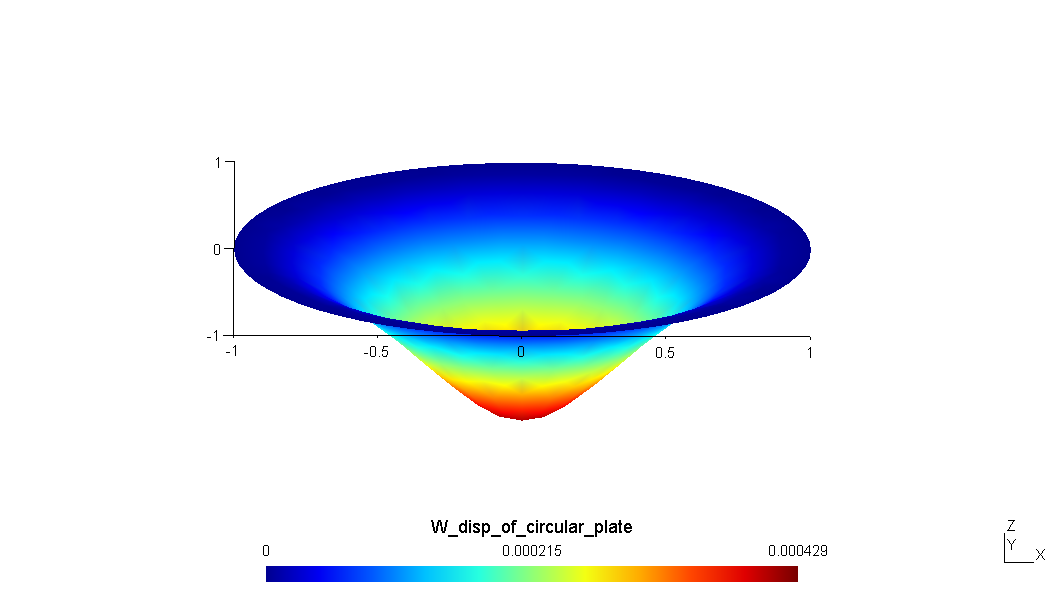
\includegraphics[width=\linewidth,trim={5cm 4cm 5cm 4cm},clip]{TIM69_pos.png}
  % \caption{FEM solution plot}
\endminipage
\end{figure}

\begin{block}{Reference}
S.Timoshenko , S . Woinowsky , Theory of Plates and Shells , pg:69, Article : 19 . 
\end{block}
Error $\%$ = 1.27 $\%$.



\end{frame}

\begin{frame}
\frametitle{VMP09}

\begin{figure}[h!]
\begin{subfigure}{.3\textwidth}
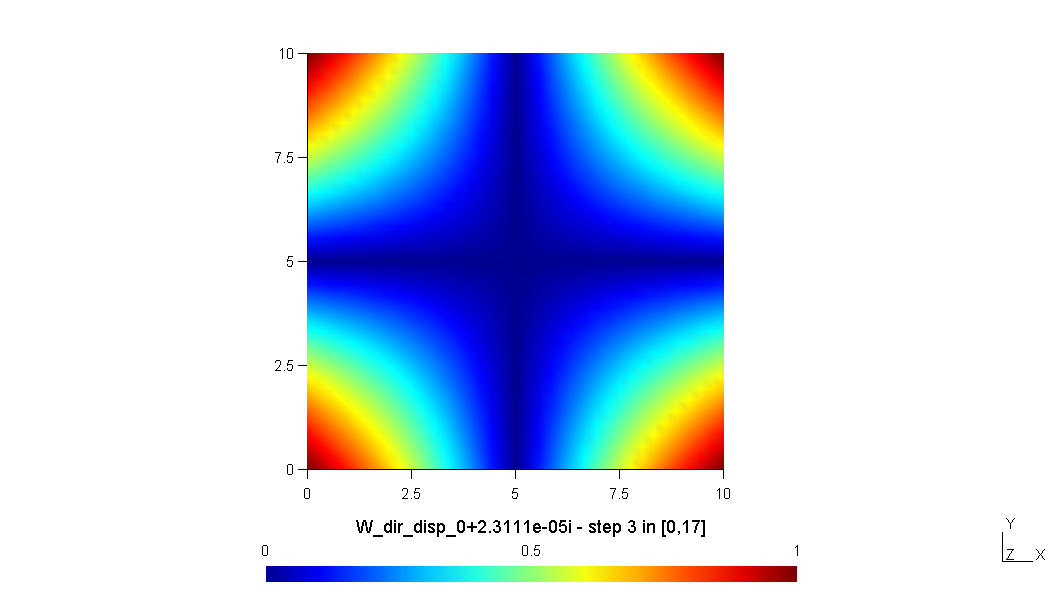
\includegraphics[width=\linewidth,trim={8cm 4cm 8cm 2cm},clip]{VMP09_T12_pos_F4.png}
%\caption{Mode Shape 4}
\end{subfigure} \hfill
\begin{subfigure}{.3\textwidth}
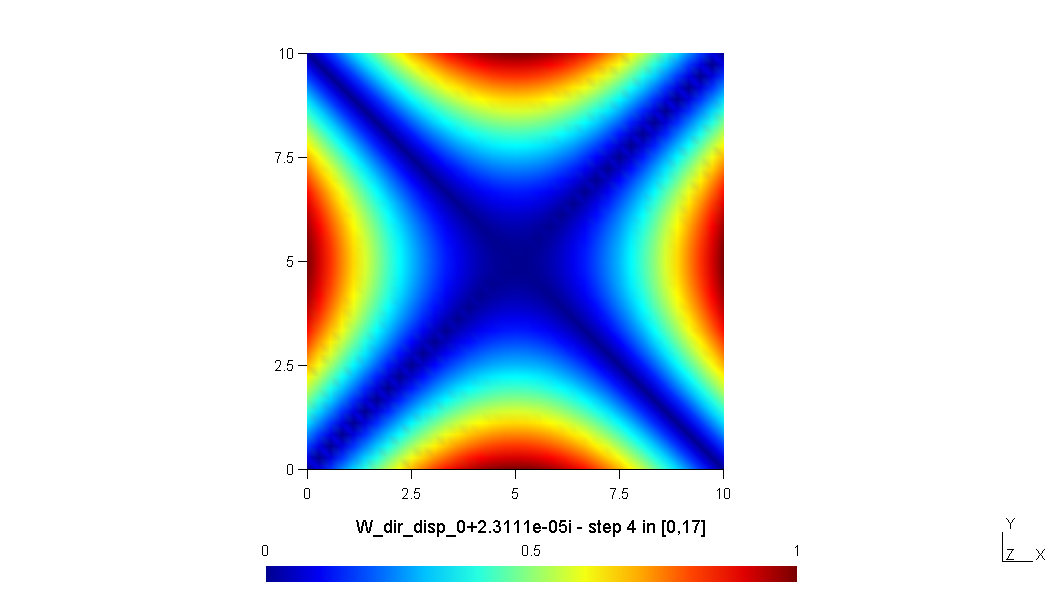
\includegraphics[width=\linewidth,trim={8cm 4cm 8cm 2cm},clip]{VMP09_T12_pos_F5.png}
%\caption{Mode Shape 5}
\end{subfigure}\hfill
\begin{subfigure}{.3\textwidth}
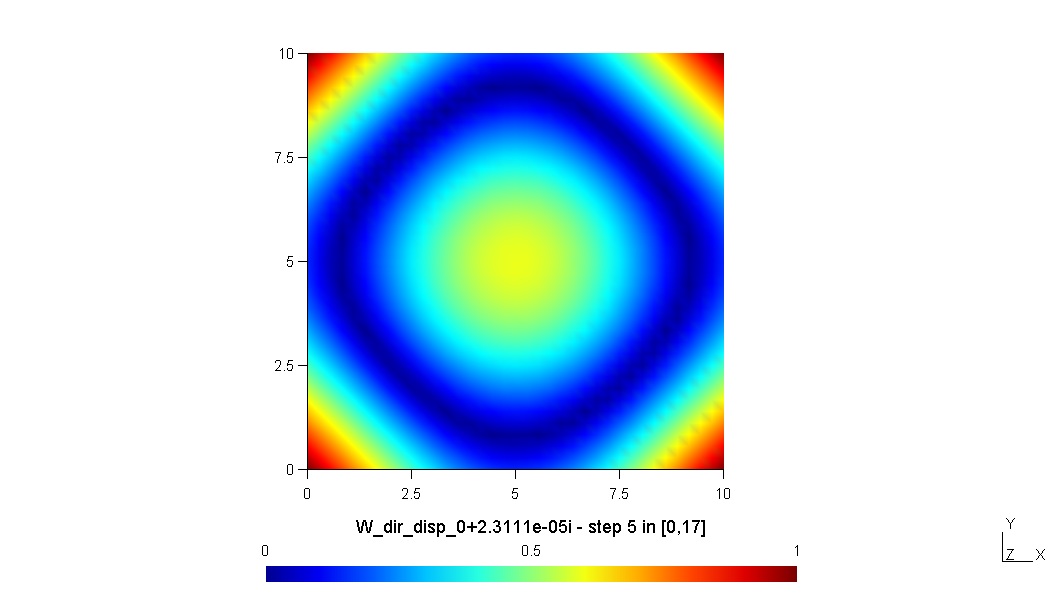
\includegraphics[width=\linewidth,trim={8cm 4cm 8cm 2cm},clip]{VMP09_T12_pos_F6.png}
%\caption{Mode Shape 6}
\end{subfigure}\vfill
\begin{subfigure}{.3\textwidth}
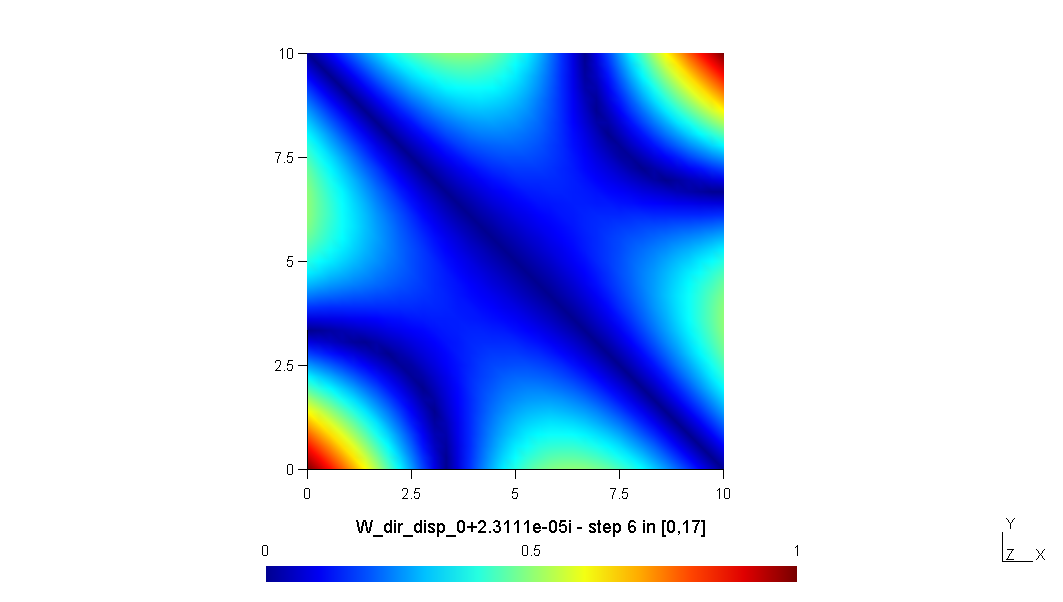
\includegraphics[width=\linewidth,trim={8cm 4cm 8cm 2cm},clip]{VMP09_T12_pos_F7.png}
%\caption{Mode Shape 7}
\end{subfigure} \hfill
\begin{subfigure}{.3\textwidth}
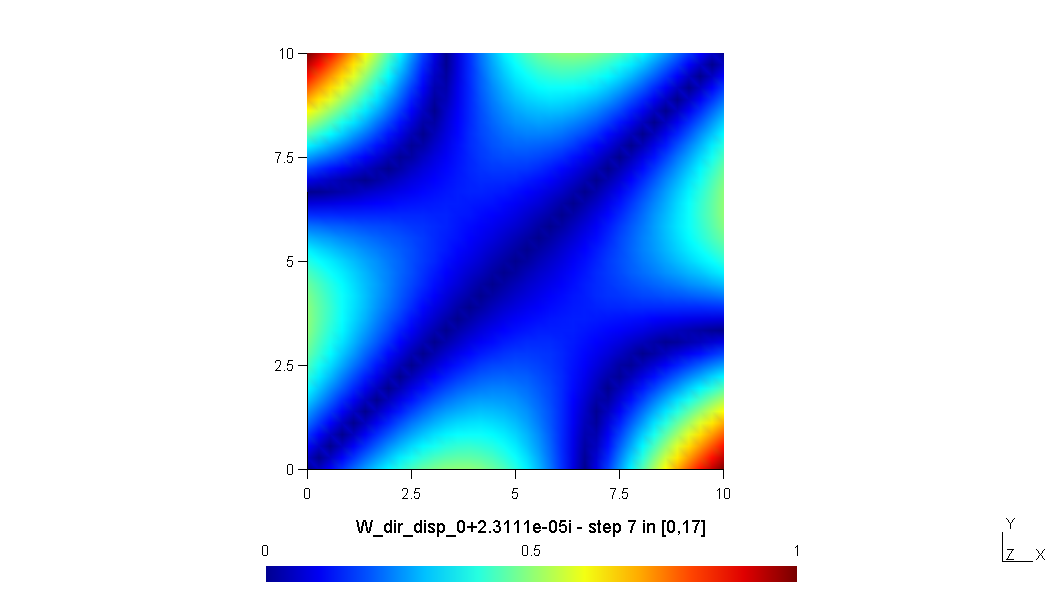
\includegraphics[width=\linewidth,trim={8cm 4cm 8cm 2cm},clip]{VMP09_T12_pos_F8.png}
%\caption{Mode Shape 8}
\end{subfigure}\hfill
\begin{subfigure}{.3\textwidth}
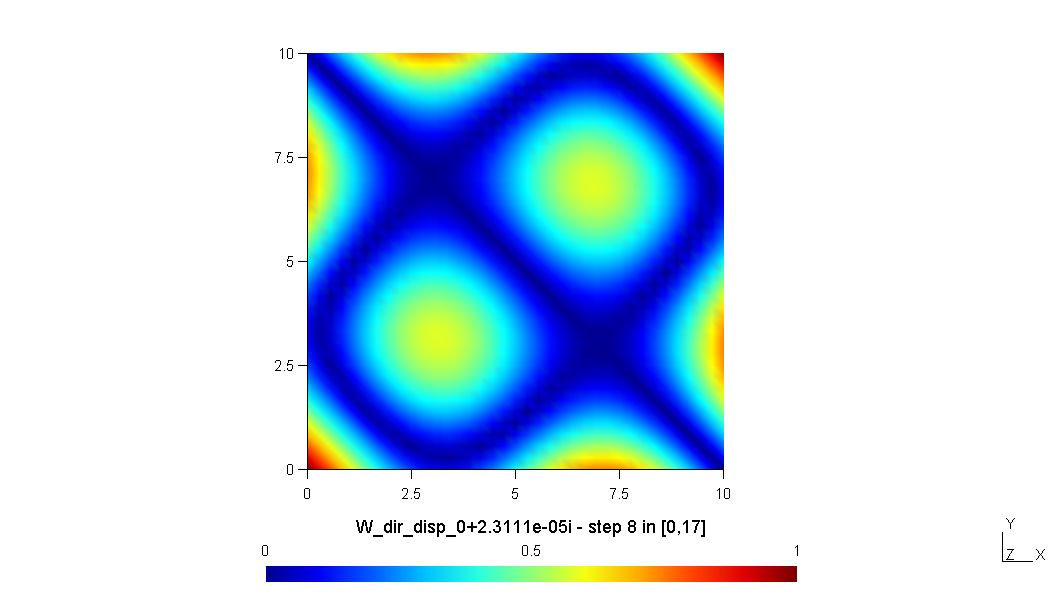
\includegraphics[width=\linewidth,trim={8cm 4cm 8cm 2cm},clip]{VMP09_T12_pos_F9.png}
%\caption{Mode Shape 9}
\end{subfigure}
%\caption{Natural Modes of a Square Plate}
\end{figure}

\begin{block}{Reference}
NAFEMS Manual. Solution Retrieved from Ansys verification problem (VMP09-T12).
\end{block}
Error $\%$ = 0.32 $\%$.



\end{frame}



\begin{frame}
\frametitle{NAS227}


\begin{figure}[h!]
\centering
\begin{subfigure}{.8\textwidth}
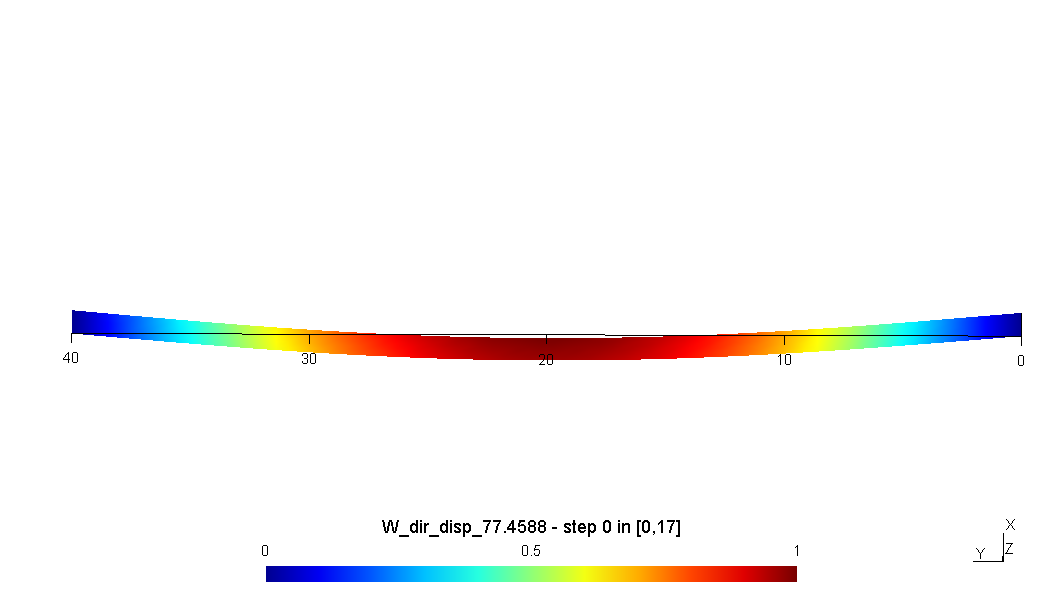
\includegraphics[width=\linewidth,trim={0 8cm 0 8cm},clip]{NAS277_pos_1.png}
%\caption{Mode Shape 1}
\end{subfigure} \vfill
\begin{subfigure}{.8\textwidth}
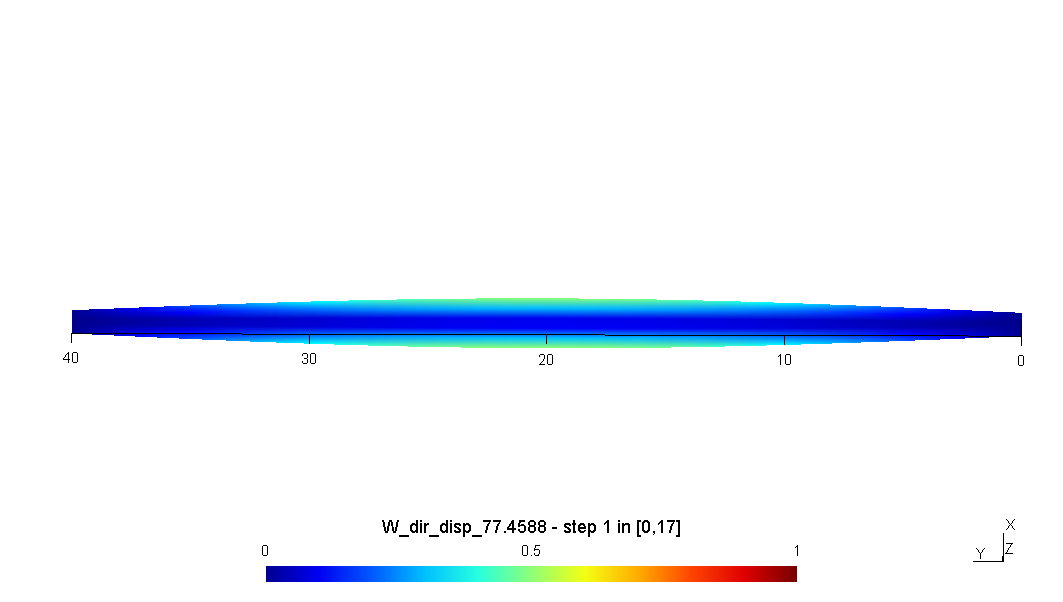
\includegraphics[width=\linewidth,trim={0 8cm 0 8cm},clip]{NAS277_pos_2.png}
%\caption{Mode Shape 2}
\end{subfigure}\vfill
\begin{subfigure}{.8\textwidth}
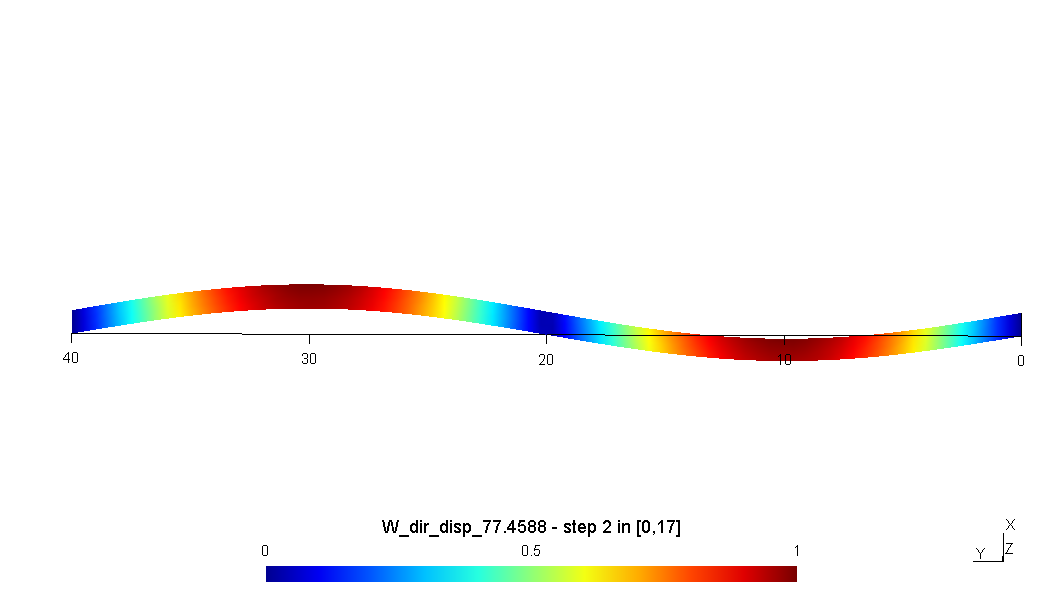
\includegraphics[width=\linewidth,trim={0 8cm 0 8cm},clip]{NAS277_pos_3.png}
%\caption{Mode Shape 3}
\end{subfigure}

%\caption{Natural Modes of a rectangular strip}
\end{figure}

\begin{block}{Reference}
Arthur W.Leissa ,Vibration of Plates,NASA SP-160, pg:277, Ch:10.2. \\
\end{block}
Error $\%$ = 0.01 $\%$.



\end{frame}



\begin{frame}
\frametitle{Wave Speed}


\begin{figure}[h!]
\centering
\begin{subfigure}{1\textwidth}
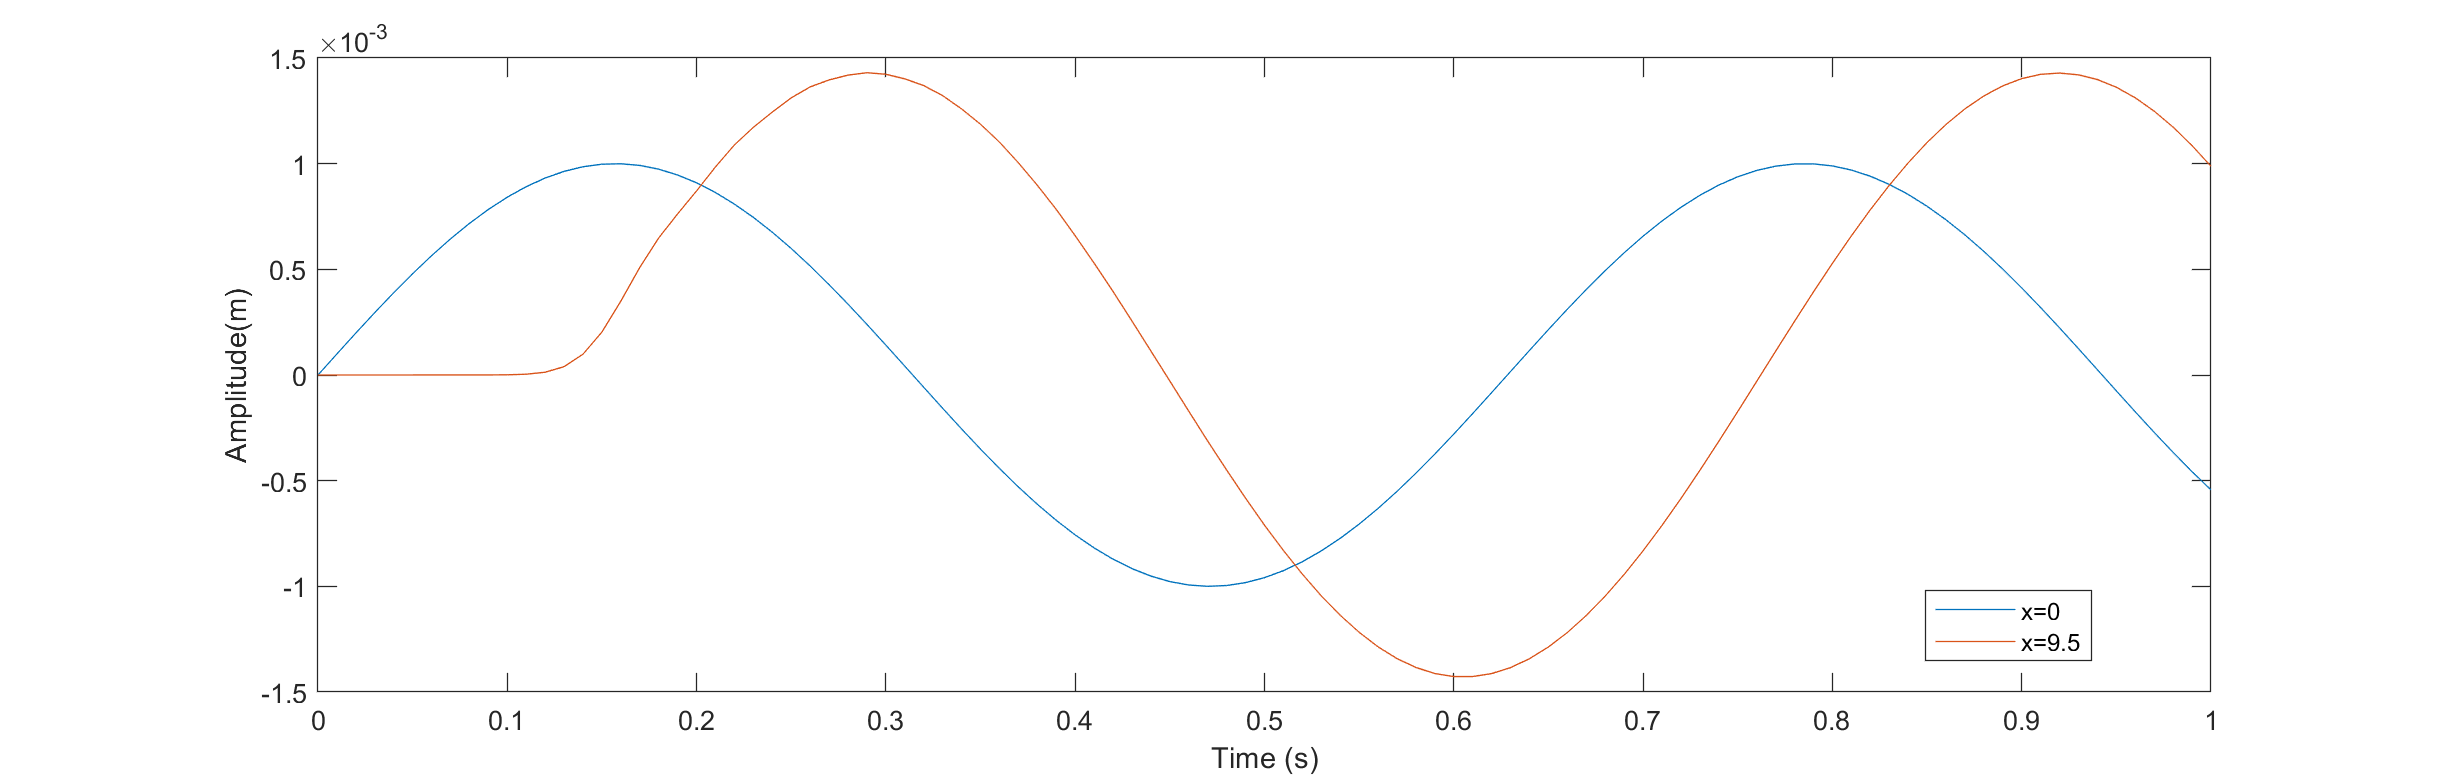
\includegraphics[width=\linewidth,trim={0 0 0 0},clip]{wavespeed.png}
%\caption{Mode Shape 1}
\end{subfigure} 

%\caption{Natural Modes of a rectangular strip}
\end{figure}

\begin{block}{Formula}
$c=v+sqrt(T/m)$ \\  $T$ = Tension , $m$ = Mass per unit length, $v$ = line speed and $c$ = wave speed. 
\end{block}
Error $\%$ = 0.89 $\%$.

\end{frame}

\begin{frame}
\frametitle{comparison with 1D FD model}
\begin{figure}[h!]
\centering
\minipage{1\textwidth}%
  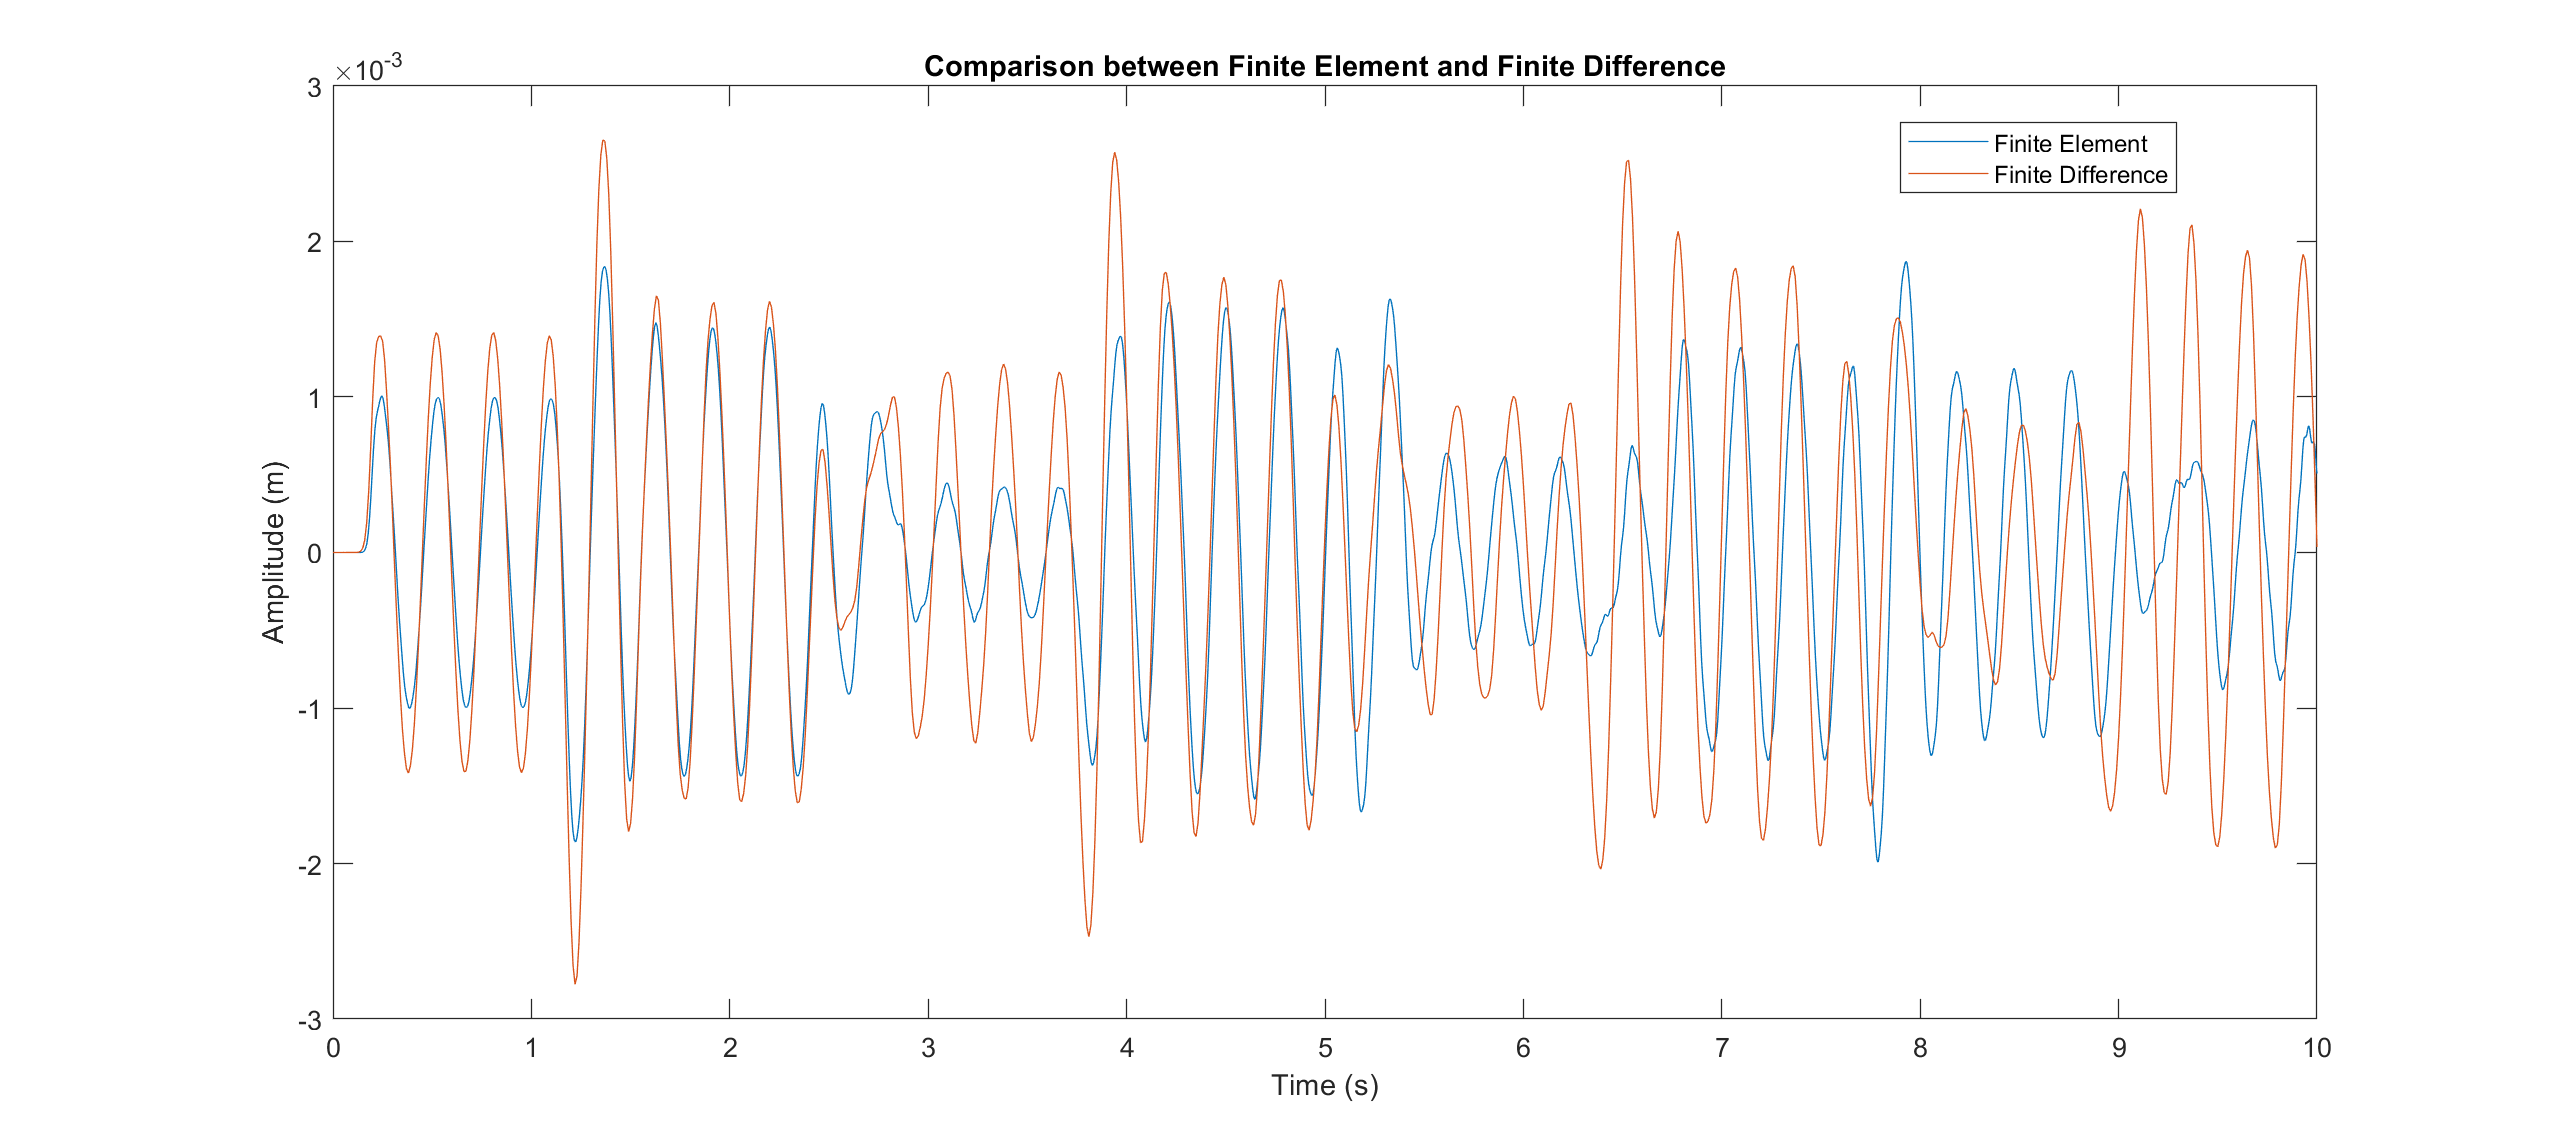
\includegraphics[width=\linewidth,trim={2cm 0 2cm 0},clip]{FdvsFe1.png}
  %\caption{FEM solution plot}\label{fig:awesome_image3}
\endminipage
\end{figure}
\end{frame}


\begin{frame}
\frametitle{Dynamic Analysis}
%\movie[width=0.7\textwidth]{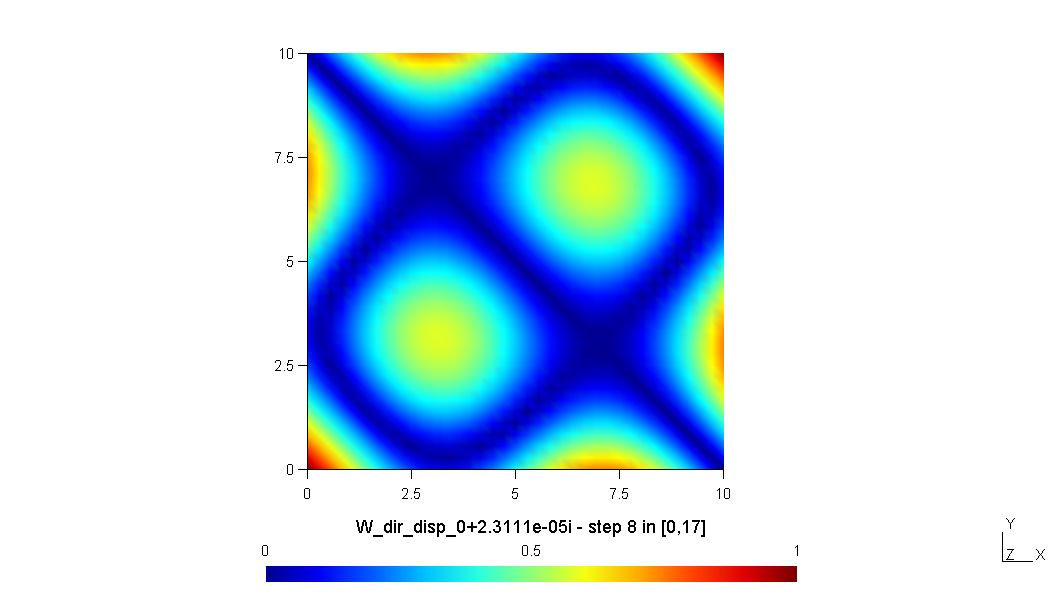
\includegraphics[width=0.7\textwidth]{VMP09_T12_pos_F9.png}}{movie1.mpg}
\begin{columns}

\column{0.5\textwidth}
\href{run:c:/Users/Admin/Desktop/documentation/presentation/movie1.mpg}{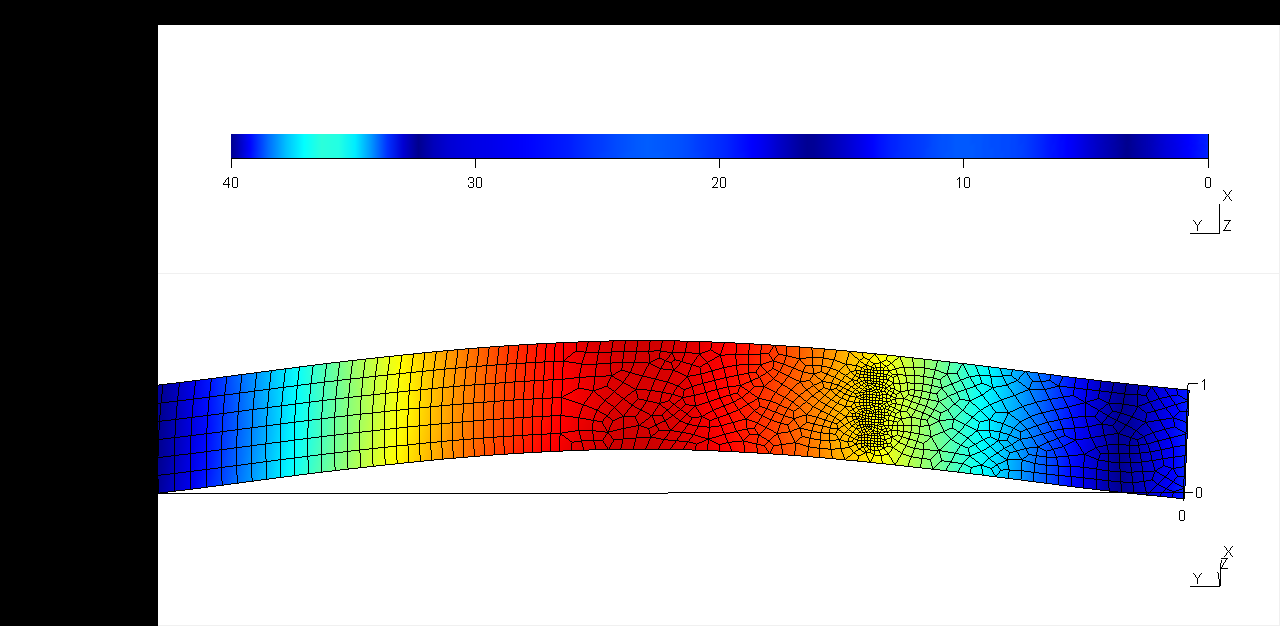
\includegraphics[width=0.7\textwidth]{movie1.png}}
\column{0.5\textwidth}
\href{run:c:/Users/Admin/Desktop/documentation/presentation/movie2.mpg}{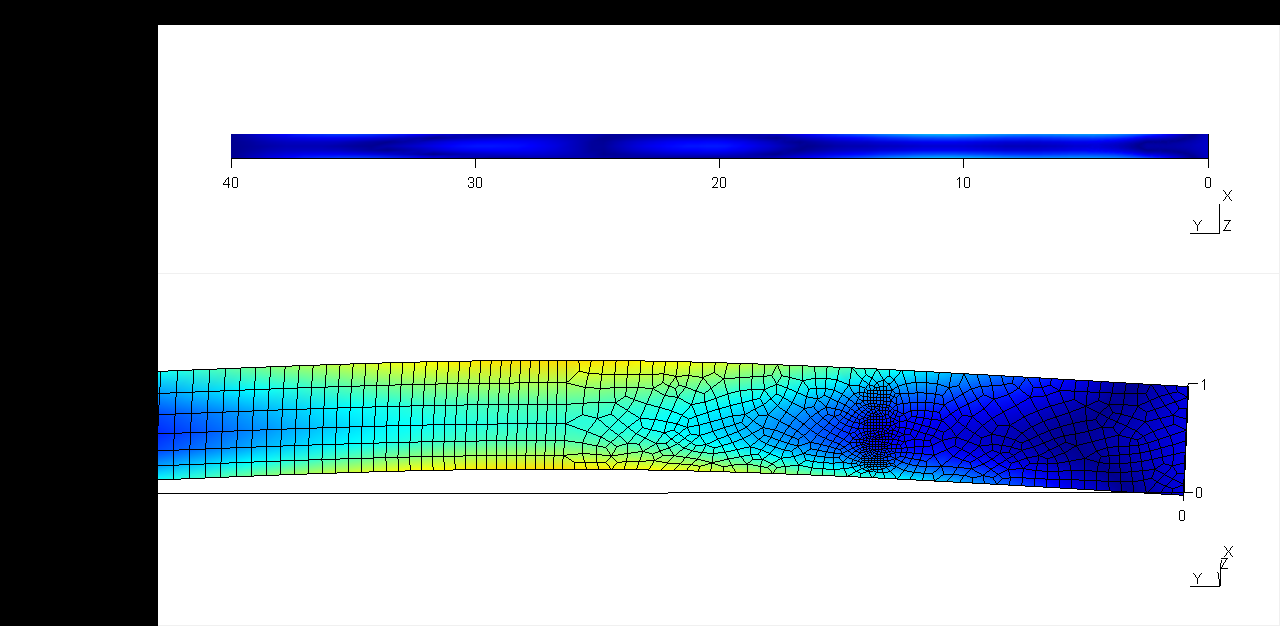
\includegraphics[width=0.7\textwidth]{movie2.png}}
\end{columns}
\end{frame}

\section{Conclusion}
\begin{frame}
\frametitle{Conclusion}
\begin{block}{Advantages of FEM}
\begin{itemize}
\item More Accurate than many numerical Methods.
\item Once coded successfully, It is very easy to implement even for complex geometry and mesh.
\item Higher dimensions can be easily modeled.
\end{itemize}

\end{block}

\begin{block}{Disadvantages of FEM}
\begin{itemize}
\item Computationally expensive.
\item Complexity in coding may be overwhelming .
\item Suffers from "The curse of dimensionality!".

\end{itemize}

\end{block}
\end{frame}

\begin{frame}
Thank you for your attention!!!
\end{frame}

\end{document}
